\documentclass[../thesis.tex]{subfiles}

\begin{document}

\chapter{Event reconstruction}
\label{chap:recon}

\section{Introduction}
\label{sec:reconIntro}

\autoref{chap:calib} discussed the process of taking the raw ADC and TDC values of PMT hits, as measured by the front-end electronics, and converting those values, channel-by-channel, into the more useful quantities of hit charge (in photoelectrons) and hit time (in, e.g., nanoseconds). The next step is to combine information from all of the channels in order to derive properties of the event as a whole, such as the amount of deposited energy and the approximate location of the vertex. This is the purpose of \emph{reconstruction.}

Reconstruction begins with the calculation of the total observed charge (i.e. photoelectron count) by summing hits across all channels, with a correction for the presence of any inactive channels. This \emph{nominal charge} is then converted into \emph{raw energy}, in MeV, according to an energy scale determined using regular (weekly or more) calibrations. At the same time, the distribution of charge across PMTs is used to estimate the location within the AD of the event. The position is then used to apply a \emph{nonuniformity} adjustment to the raw energy, to correct for the position-dependent response of the detector. This gives the \emph{reconstructed energy}, which is used in most subsequent analysis stages.

The reconstructed energy should not be regarded as the best estimate of the true energy deposited by the event, given the complexities involved in the nonlinearity of the scintillator and its varying responses to different particle types. Rather, reconstructed energy should be considered a \emph{position-corrected measure of the total observed amount of light}, and hence should be regarded as proportional to the total amount of light produced in the scintillator. Due to the calibration methods used, reconstructed energy \emph{does} agree (by construction) with deposited energy for the 8~MeV gamma ray cascade from nGd capture, but this is only a special case.

Daya Bay has developed multiple independent reconstruction algorithms. The two that have been widely used in published results are known as AdSimple and AdScaled. They differ primarily in their calibration procedures, their vertex reconstruction algorithms, and their methods of correcting for nonuniformity. Both give consistent results in the oscillation analysis, and both will be detailed in this chapter, but only AdSimple will be used in our analysis.

\section{Energy reconstruction}
\label{sec:reconEnergy}

\subsection{Event charge determination}
\label{sec:reconEnergyCharge}

\subsubsection{Hit selection}
\label{sec:reconHitSelection}

The first step in the energy reconstruction is to estimate the total \emph{charge}, i.e., number of photoelectrons, observed from the underlying interaction. Here, the main consideration is the choice of hits to include in the sum. Based on the design of the trigger electronics, a trigger will be issued about \SI{1550 \pm 50}{ns} after the accumulation of a sufficient number of hits and/or total charge. Including an additional spread of 50~ns to account for the time-of-flight of the photons, one would infer that a window of around [-1650, -1450]~ns would be reasonable.\footnote{Here, as in previous discussions, the origin of time ($t = 0$) is the instant at which the trigger is issued. Since all of the recorded hits occur prior to the trigger, their time values are negative.} In practice, Daya Bay actually uses a window of [-1650, -1250]~ns. The justification for this wider window is related to the properties of the liquid scintillator itself.

When an interaction deposits energy in the LS, various molecular excited states decay stochastically, emitting light in the process. In the Daya Bay LS, the light emission can be accurately modeled with three components: a fast one ($\sim$5~ns time constant), a medium one ($\sim$30~ns), and a slow one ($\sim$150~ns). The time for light to propagate, directly or via reflections, adds a position-dependent delay of a few dozen ns. Altogether, 5\% of the PMT hits occur some 50-150~ns after the primary peak \cite{peakCharge}. In order to include this ``late'' light, and thereby hopefully improve the energy resolution, Daya Bay uses the widened hit selection window of [-1650, -1250]~ns.

With a window defined for hit selection, the next question is which hits to use from inside this window. Based on the measures discussed in \autoref{sec:calibHitCharge} for correcting the biases in closely-spaced hits, in principle every hit should be trustworthy. In practice, hits that arrive within 100~ns of each other will produce a single shaped peak, and hence only the first hit will have a nonzero calibrated charge. Since most primary light hits \emph{do} in fact arrive within 100~ns of each other, there is usually no difference between taking all hits and taking only the first hit. The \emph{default} or \emph{nominal} charge is accordingly defined as \emph{the sum across channels of the earliest hit in the time window of [-1650, -1250]~ns (relative to the trigger time).}

The nominal charge will generally account for all of the fast/medium light, but will omit \emph{some} of the slow light \emph{unless there is no fast/medium light seen by the channel}. As such, high-energy events will miss a greater proportion of slow light compared to low-energy events, since in the latter case there will be more channels seeing no fast/medium light. This introduces a degree of nonlinearity in the overall detector response. If, instead, one were to take \emph{all} hits in [-1650, -1250]~ns, instead of just the earliest hit, the sum would in principle accurately include all of the components, without the aforementioned nonlinearity. This does not appear to have ever been proposed; the reasons are unknown, but may be related to the fact that this method is more sensitive to the details of the corrections for closely-spaced hits.\footnote{%
However, there \emph{was} an alternative to the nominal charge that was discussed for a time in the earlier days of the experiment. The \emph{peak charge} was defined as the sum across channels of the earliest hit in [-1650, -1480]~ns. This time window effectively excludes the late light, and thus mitigates the associated nonlinearity found in the nominal charge. One (perhaps insignificant) downside of the peak charge is that it includes slightly less light, but late light accounts for only 5\% of the total, and the nominal charge misses some of it anyway, so the overall loss of photon statistics is only on the order of a couple percent. Most likely, in the author's opinion, is that the nominal charge was retained primarily due to inertia. In any case, it is possible to measure and correct for any nonlinearity inherent in the charge calculation, as discussed in \autoref{sec:reconEnergyNL}, so there is a degree of latitude in choosing from among these various methods.%
}


\subsubsection{Active channel correction}
\label{sec:reconActiveChan}

At any given time, there may be dead or malfunctioning channels in an AD. As described in \autoref{sec:calibCQ}, these are recorded in the channel quality (CQ) database according to a number of criteria. If, at the time of a given trigger, a channel is marked as ``bad'', then its charge is \emph{not} included in the total nominal charge. This, naturally, will result in a downward bias on the total. In principle, the size of the effect depends on the position of the event: The effect is larger if the event is closer to the PMT, and vice versa. In practice, however, Daya Bay uses a simple, position-independent correction of $192/N$, where $N$ is the number of active channels. Given that the Daya Bay ADs almost always have fewer than two bad channels, this correction was found to reliably correct the bias, with negligible impact on the resolution.

\subsubsection{Summary}
\label{sec:reconChargeSummary}

In summary, the nominal charge is computed as follows: For every active channel, take the calibrated charge of the earliest hit in the window of [-1650, -1250]~ns pre-trigger. Sum these up, and then apply a correction of $192/N$, where $N$ is the number of active channels. In subsequent stages of the energy reconstruction, the nominal charge (in PE) is scaled by a time-dependent energy scale to give the \emph{raw energy} (in MeV), then adjusted by a time- and position-dependent nonuniformity correction to give the \emph{reconstructed energy} and, finally, at the highest levels of analysis, adjusted again to correct for electronics nonlinearity, scintillator nonlinearity, and IBD kinematics to give the \emph{true neutrino energy}. These steps are discussed below.

\subsection{Energy scale calibration}
\label{sec:reconEnergyScale}

The nominal charge produced by a given interaction can vary over time due to, for instance, degradation or contamination of the scintillator. Furthermore, for the purpose of physics analysis, we would prefer to speak of the energy (in, e.g., MeV) deposited in the scintillator, rather than the amount of light observed. Accordingly, the object of the energy scale calibration is to fix the definition of a ``visible'' MeV, and to ensure that any given event will yield the same reconstructed energy in every AD, regardless of changes over time in the behavior of the scintillator.

In what follows, repeated references will be made to the so-called \emph{Crystal Ball (CB) function} \cite{cbfunction}. This empirical function was initially developed by the Crystal Ball collaboration, which operated a neutral particle detector (containing an inner spark chamber surrounded by a sphere of scintillating crystals) at SLAC around the early 1980s. The CB function is designed to model ``lossy'' processes, such as energy deposition in a detector where some energy can escape detection. At Daya Bay, neutron capture on gadolinium provide an example of such a process, as gamma rays may exit the scintillating volume before depositing all of their energy. To account for both fully and partially contained events, the CB function includes a Gaussian ``core'' and a power-law ``tail'', respectively:
\begin{equation}
  \label{eq:cbfunction}
  f(x;\alpha,n,\bar x,\sigma) = N \cdot \begin{cases} \exp(- \frac{(x - \bar x)^2}{2 \sigma^2}), & \mbox{for }\frac{x - \bar x}{\sigma} > -\alpha \\
    A \cdot (B - \frac{x - \bar x}{\sigma})^{-n}, & \mbox{for }\frac{x - \bar x}{\sigma} \leqslant -\alpha,\end{cases}
\end{equation}
where
\[
  A = \left(\frac{n}{\left| \alpha \right|}\right)^n \cdot \exp\left(- \frac {\left| \alpha \right|^2}{2}\right),%
  \qquad%
  B = \frac{n}{\left| \alpha \right|}  - \left| \alpha \right|,
\]
and $N$ is a normalization factor. In the case of fitting the energy spectrum of nGd captures, we will be discussing the use of a \emph{double Crystal Ball function}, that is, the sum of two CB functions, one of which fits the 7.937~MeV peak from capture on $^{157}$Gd, and the other of which fits the 8.536~MeV peak from $^{155}$Gd. Among the isotopes of Gd with significant neutron capture cross sections, these two are the most abundant in natural Gd.

Given that the response of the ADs (i.e. the nominal charge) depends on the type of interaction and is nonlinear with respect to the deposited energy, the energy scale (in charge per MeV) will depend on the choice of interaction used to calibrate the scale. Daya Bay's two main reconstruction algorithms, AdSimple and AdScaled, both define the energy scale such that a neutron capture on gadolinium will yield approximately 8 MeV\footnote{More precisely, the energy scale is defined such that the nGd capture spectrum contains two peaks (as fit by a double Crystal Ball function) at reconstructed energies of 7.937 and 8.536~MeV. In principle, the nonlinearity of the detector could mean that if the first peak is fixed at 7.95~MeV, the second might not lie exactly at 8.54~MeV, suggesting that the spacing between the two peaks should be allowed to float in the fit. In practice, however, at such high energies, the degree of nonlinearity (relative to the energy resolution) is insufficient to compromise the fit, and so a fixed peak spacing is used.}. However, there are significant differences between the methodology of the two calibrations.

For AdSimple, the calibration uses Gd captures of spallation neutrons produced by high-energy cosmic muons traversing the AD. Since this analysis is based on AdSimple, we give a detailed description of its calibration procedure in the section that follows. One of the advantages of using spallation neutrons is that they are distributed uniformly throughout the target volume, much like IBD neutrons. A disadvantage is that the ensuing energy scale is slightly biased (upward), relative to that of IBD neutrons, due to PMT afterpulsing resulting from the large amount of charge produced by the parent muon. In the end, however, this is accounted for in the nonlinearity model (\autoref{sec:reconEnergyNL}); as long as the energy scale calibration provides consistency in time, space, and between ADs, it is sufficient.

In comparison to AdSimple, AdScaled uses a significantly different method of calibrating the energy scale. We only discuss it briefly, since AdScaled is not used in this analysis. Essentially, the method is based on using weekly $^{60}$Co calibrations to monitor the time variation of the light yield, and occasional $\sim$40-hour AmC calibrations (which produce nGd captures) to measure the nonlinearity between the $^{60}$Co and nGd peaks. Every Friday, the $^{60}$Co source is deployed from ACU A to the center of each AD for 10 minutes. From this data is extracted a histogram containing the total nominal charge of each event. In the vicinity of the $^{60}$Co peak, this histogram is fit to a Gaussian plus Crystal Ball function \cite{adScaledTechnote}. The nominal charge (at the peak of the fit function) is then multiplied by the ratio between the nGd and $^{60}$Co charge peaks\footnote{This ratio, which is relatively stable, is determined from runs in which the $^{60}$Co and $^{241}$Am-$^{13}$C sources are deployed together at the center of the AD. In the nominal charge spectrum from such a run, the $^{60}$Co peak is fit, as above, to a Gaussian plus Crystal Ball. Meanwhile, the nGd peak is fit to a simple Gaussian \cite{adScaledTechnote}; since the nGd captures occur at the detector's center, the gamma leakage tail is very small, allowing the use of a Gaussian instead of a (double) Crystal Ball. (Of course, the same reasoning would permit the use of a simple Gaussian for $^{60}$Co as well. The authors of AdScaled nonetheless chose the more complicated function in production, even though they found a simple Gaussian to work well during testing.) Once both peaks have been fit, the ratio in question is simply the ratio of the two peaks as defined by the best fits.}, as determined by the nearest long AmC run, and this scaled light yield is stored in the database for use by the reconstruction. This method works because the \emph{ratio} of the nGd and $^{60}$Co peaks is quite stable, even when the peaks themselves are varying. (Omitting $^{60}$Co, and using AmC alone, would avoid the need for this scaling, but the rate of neutrons from the AmC source is insufficient to provide the necessary statistics.) It is worth noting that the resulting energy scale is defined in terms of events at the \emph{center} of the AD, rather than uniformly distributed throughout the GdLS (as in AdSimple). This leads to a consistent $\sim$5\% difference in the energy scale calibration constants between the two algorithms. Essentially, this is only a difference in conventions (i.e., defining the energy scale based on uniformly distributed vs. centered events), which is accounted for at the event-by-event level by the nonuniformity correction, as discussed in \autoref{sec:reconEnergyNU}.

\begin{comment}
  A sample enriched in such neutrons is obtained by selecting events in a time window (XXX define) immediately after AD muons (XXX of what minimum energy?). These captures are distributed uniformly throughout the GdLS, much like IBDs. The nGd capture peak in the charge distribution is fit to a Gaussian (XXX crystal ball?), and the location of the peak is defined as corresponding to 7.95 MeV (XXX) 8.0 MeV according to doc-7334 (AdSimple). This energy scale is stored in the offline database, valid for the period in which the neutrons were collected. In the near (far) halls, it takes XXX (YYY) days to obtain the necessary statistics; this is thus the time-resolution of the energy scale, which is sufficient, given that the light yield changes very slowly, declining by some 1\% to 1.5\% per year.
  
24 hours
\end{comment}

\begin{comment}
  Figure out exactly what energy is pegged by AdSimple and AdScaled. 7.95 MeV? Discuss differences (e.g. due to muon afterpulsing?)
  5x15min Co60
  4x10hour AmC
\end{comment}

\subsubsection{AdSimple calibration procedure}
\label{sec:reconEnergyAdSimpleCalib}

The AdSimple energy calibration begins with the selection of a sample of spallation neutron candidates. These are defined based on their proximity in time to a preceding AD muon, where an AD muon is regarded as any event that produces more than 3,000 photoelectrons of nominal charge. Non-muon events are filtered through a simplified cut to remove instrumental backgrounds (``flashers''); specifically, the \emph{ellipse cut} described in \autoref{sec:bkgFlashers} is employed (\autoref{eq:ellipseCut}). For any surviving event with a nominal charge of more than 100 PE (roughly 0.6~MeV), the charge (after correcting for any dead PMTs, as described in \autoref{sec:reconActiveChan}) is added either to a \emph{signal} histogram, if the time since the previous muon is between 20 and \SI{1000}{\micro s}, or to a \emph{background} histogram if $\Delta t$ is between 1020 and \SI{2000}{\micro s}\footnote{The \SI{20}{\micro s} gap between the two windows ensures that both windows are of the same length. Alternatively, a background window of 1000 to \SI{1980}{\micro s} could have been used, etc.}. Given that the characteristic nGd capture time is $\sim$\SI{30}{\micro s}, the latter histogram provides a clean sideband measurement of the background spectrum.

\begin{comment}
  Note: For AdSimpleNL, in reconstruction, a (AD-specific?) scale constant is applied to the non-NL energy scale constant. See line 209 of QsumEnergyTool.cc. Discuss this?
\end{comment}

These histograms are stored in files that correspond one-to-one with Daya Bay DAQ files (each spanning roughly ten minutes in one hall). The files are processed sequentially, and for each AD, a new energy scale constant is calculated once 10,000 entries have been accumulated in the background\footnote{From the sideband.}-subtracted histogram of spallation neutron charges. The constant is determined by fitting the charge spectrum to a double CB function, whose two components, as discussed previously, correspond to the peaks from neutron capture on $^{155}$Gd and $^{157}$Gd. The relationship between the two CB functions (``peaks'') is constrained as follows:

\begin{enumerate}
\item The shape parameters $\alpha$ and $n$ are the same, and constrained to lie within (0, 5) and (0, 1), respectively.
\item The amplitude of the $^{155}$Gd peak is constrained to be 0.227 of the $^{157}$Gd amplitude, according to the product of the relative abundances (14.80\% and 15.65\%, respectively) and neutron capture cross sections (60,700 and 257,000 barns, respectively \cite{doi:10.13182/NSE05-64}) of the two isotopes.
\item The location of the $^{155}$Gd peak is constrained to be 1.0755 of that of the $^{157}$Gd peak, based on the total gamma ray energies of 8.536 and 7.937~MeV emitted after neutron capture on the two isotopes.
\item The two $\sigma$ (width) parameters are related by the square root of the aforementioned ratio of peak locations.
\end{enumerate}

After the fit is performed, the location parameter $\mu$ of the first peak (generally between 1200 and 1350~PE) is assumed to correspond to 7.937~MeV (from $^{157}$Gd), and so, in this convention, the energy scale constant is simply $\mu/7.937$ PE/MeV. However, due to the PMT afterpulsing that occurs after a high-energy muon event, this value is biased upward compared to the energy scale for the IBD nGd captures. This would not be issue if the bias were the same size in all halls (since it could then simply be absorbed into a common nonlinearity correction), but because the muon rate and spectrum differ between halls, so does this bias. Such a systematic difference in energy scales could bias the oscillation fit. Accordingly, the energy scales are corrected by an AD-specific factor (ranging from 0.9895 to 0.9934), empirically determined in order to match the IBD-nGd energy scale in the extrapoloated limit of zero muon energy \cite{spallScaleCorr}. These corrected energy scales are stored in the database for use by the AdSimple reconstruction.

\subsection{Nonuniformity correction}
\label{sec:reconEnergyNU}

Given the nominal charge $Q$ and the energy scale $S$, the \emph{raw visible energy} $\Eraw$ is simply $Q/S$. Given that the light collection efficiency differs as a function of position within the AD, the effective energy resolution would be degraded if $\Eraw$ were directly used in physics analysis. Fortunately, this nonuniformity can be measured and corrected for. In the case of AdSimple, the current nonuniformity map was produced from three years of data by dividing the AD into pixels (in $R^2$ and $Z$) and selecting spallation neutron captures on both gadolinium and hydrogen within each pixel. For each pixel within the GdLS, the nGd spectra was fit to a double Crystal Ball function (along with an additional exponential tail, found to improve fit quality), and the location of the peak was divided by the mean nGd peak among all GdLS pixels, giving the correction factor. (This choice of denominator reflects the fact that the energy scale is determined using events uniformly distributed within the GdLS). Meanwhile, for each LS pixel, the nH peak was fit to the ``Daya Bay Function'' (a specific case of the general \emph{Calorimeter Function} developed by members of the collaboration \cite{dybfunction}):
\begin{equation}
  \label{eq:dybfunction}
  \begin{aligned}
    f_{\mathrm{DYB}}(E) = \; & N_\mathrm{peak} \cdot \frac{1}{\sigma \sqrt{2\pi}} e^{-\frac{(E-\mu)^2}{2\sigma^2}} \\
    & + N_{\mathrm{tail}} \cdot \left\{ \frac{\lambda}{2} e^{\frac{\sigma^2\lambda^2}{2}}
    e^{\lambda E} \left[ \erf\left( \frac{\mu-(E+\sigma^2\lambda)}{\sqrt{2}\sigma} \right) - \erf \left( \frac{0 - (E+\sigma^2\lambda)}{\sqrt{2}\sigma} \right) \right] \right.\\
    & \phantom{ + N_{\mathrm{tail}} \cdot } \left. \quad+\frac{a}{2} \left[ \erf\left( \frac{\mu-E}{\sigma\sqrt{2}} \right)  - \erf \left( \frac{0-E}{\sigma\sqrt{2}} \right)\right]\right \}.
  \end{aligned}
\end{equation}
This function has six parameters: The normalizations $N_{\mathrm{peak}}$ and $N_{\mathrm{tail}}$, the peak location $\mu$, the peak width $\sigma$, and the two tail shape parameters $\lambda$ and $a$. In a given pixel, the fitted peak $\mu$ was divided by the mean nH peak among all \emph{GdLS} pixels \cite[p. 20]{yuryNonUni} to obtain the pixel's nonuniformity factor.

Within AdSimple, the reconstructed vertex position (\autoref{sec:reconVertex}) was looked up (using bilinear interpolation) in this nonuniformity map, and the resulting (time-invariant) correction factor was applied. However, it has been shown that the nonuniformity of the AD changes over time (along with the energy scale), presumably because decreases in the attenuation length of the scintillator will proportionally affect events located near the edge of the AD, compared with events near the center. This behavior was found to be consistent between all ADs, and adequately captured by the simple analytical expression \cite[p. 16]{yuryNonUni2}:
\begin{equation*}
  \frac{\Delta E}{E} = (a + b R^2)\, \Delta t,
\end{equation*}
where
\begin{align*}
  a &= -0.00149 \pm 0.00030,\\
  b &= 0.00109 \pm 0.00013,
\end{align*}
$R$ is the radial coordinate (in meters) of the event, and $\Delta t$ is the time (in years) since the mean timestamp in the data period used when generating the static nonuniformity map. Computing the corrected energy $E_{\mathrm{corr}}$ (i.e. $\Erec$) from the uncorrected energy $E_{\mathrm{uncorr}}$ then involves simply undoing this energy shift:
\begin{equation*}
  E_{\mathrm{corr}} = \left( 1 - \left.\frac{\Delta E}{E}\right|_{E=E_{\mathrm{uncorr}}} \right) \cdot E_{\mathrm{uncorr}}
\end{equation*}
After applying the full (static $\times$ time-dependent) nonuniformity correction, the resulting reconstructed energy $\Erec$ was stored in the processed data file for use in analysis.

\subsection{Nonlinearity correction}
\label{sec:reconEnergyNL}

  Although $\Erec$ provides a reliable, repeatable, position- and time-independent proxy for the energy of an interaction, it is \emph{not} simply linearly proportional to the actual deposited energy. By construction, AdSimple's $\Erec$ will report the correct deposited energy for the $\sim$8~MeV gamma ray peak produced by nGd capture. However, due to differences in scintillator response to positrons versus gamma rays, $\Erec$ will report a different value for a \emph{positron} that deposits 8~MeV. Furthermore, even when considering a single type of particle, the combined response of the scintillator and the electronics varies by some 10\% across the range of energies used in the analysis (0.7--12~MeV). If this nonlinearity is not corrected for, then the resulting distortion in the IBD positron spectrum will potentially bias the extraction of $\Dmsqee$. The purpose of the nonlinearity correction is thus to compensate for the scintillator and electronics nonlinearity\footnote{The nonlinearity correction is not actually performed during reconstruction. Instead, the correction is applied by the fitter (\autoref{chap:fitting}), which takes AdSimple's $\Erec$ and converts it into $\Enu$. However, as this is merely an implementation detail, we discuss the conversion in this chapter, along with the other preceding steps of the energy reconstruction.}, yielding the ``true'' deposited energy $\Edep$ (assuming a positron event\footnote{Given that, for the purpose of oscillation physics, the IBD positron spectrum is the only one whose shape carries any significance, there is no need in this analysis to apply separate corrections for purported gamma ray, electron, or alpha particle events. Indeed, the delayed (i.e. nGd gamma ray) spectrum does not undergo any nonlinearity correction here.}), which can then be trivially converted to the true neutrino energy, $\Enu$, using \autoref{eq:enuToEdep}:
\begin{equation*}
  \Enu \simeq \Edep + \SI{0.80}{MeV} 
\end{equation*}
Note that, in what follows, the phrase ``positron energy'' refers not to the positron kinetic energy $E_{\mathrm{kin}}$, nor to to the relativistic (i.e. mass + kinetic) energy $E_{\mathrm{rel}}$, but rather to the total \emph{deposited} energy (including annihilation gammas); that is, ``positron energy'' = $\Edep = E_{\mathrm{kin}} + 2m_e = E_{\mathrm{rel}} + m_e$. Henceforth, $\Edep$ will refer to the true deposited energy of positrons, unless a different particle is indicated in the subscript.

As was mentioned, the nonlinearity of the AD response can be divided into contributions from the scintillator and from the electronics. Both effects are on the scale of 10\%, and work in opposite directions: The scintillator response is suppressed for low-energy events, while the electronics show a reduced response for high-energy events. Nevertheless, they do not cancel each other very effectively, so each must be treated separately and carefully. We begin with the scintillator. In what follows, we define $\Evis$ to be (proportional to) the amount of light produced in the scintillator. In terms of physical processes, the (particle and energy-dependent) scintillator nonlinearity determines $\Evis$ from $\Edep$, and then the (charge-dependent) electronics nonlinearity determines $\Erec$ from $\Evis$. In analysis, this logic is reversed in order to determine $\Edep$ given $\Erec$\footnote{Recall that any effects from geometric nonuniformity have already been removed in the computation of $\Erec$.}.

\begin{figure}[h]
  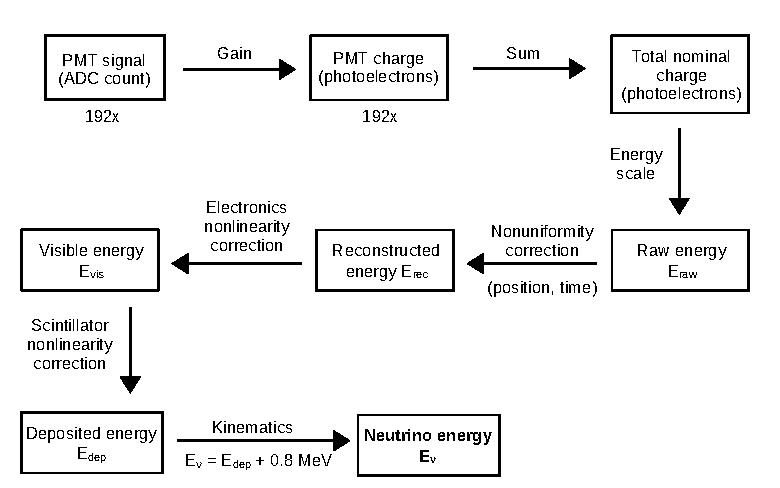
\includegraphics[scale=1.0]{Reconstruction/pmt2etrue_flow.pdf}
  \caption{Conceptual flowchart of the AdSimple energy reconstruction process. In practice, the electronics and scintillator nonlinearity corrections are applied in a single step, using the correction function described in \cite{NonlinearityPaper}. An alternative reconstruction, known as AdSimpleNL, corrects for the electronics nonlinearity at the level of individual channels, prior to summing of the charges to obtain the nonlinearity-corrected nominal charge (``NominalChargeNL''). Both methods produce consistent results. Here, we use the more ``traditional'' AdSimple algorithm.}
  \label{fig:pmt2etrue}
\end{figure}

Within the scintillator, there are two primary sources of nonlinearity: \emph{quenching} \cite{Birks_1951} and \emph{Cerenkov radiation} \cite{cerenkov}. Quenching occurs when the local ionization density is high, allowing fluorescently excited molecules to be ``quenched'' by excited neighbors, preventing light emission. Ionization density is highest when a particle is moving slowly (especially when it is near the end of its range), so, for a low-energy particle, a greater fraction of light will be quenched in comparison to a higher-energy particle, leading to nonlinear light emission as a function of energy. For organic scintillators such as the Daya Bay LS, this behavior is quantitatively well described by \emph{Birks' law} \cite{Birks_1951},
\begin{equation}
  \frac{dQ}{dx} \propto \frac{\frac{dE}{dx}}{1 + k_B \frac{dE}{dx}}
  \label{eq:reconBirks}
\end{equation}
where $Q$ is the amount of emitted light, $dE/dx$ is the linear density of \emph{ionization} energy deposition, and the scintillator-specific value $k_B$ is known as Birks' constant.

If the $dE/dx$ profile is known across a particle's range, then it can be used to integrate \eqref{eq:reconBirks}. Such a ``semi-empircal'' analytic approach was used to compute the shape of the quenching curve for electrons in the Daya Bay LS \cite{NonlinearityPaper}. This relationship was encoded in a function denoted $f_q(\Edepelec, k_B)$, where $k_B$ remained to be determined from data:
\begin{equation}
  f_q(\Edepelec,k_B) = \int_0^{\Edepelec} \frac{\frac{dE}{dx}}{1 + k_B \frac{dE}{dx}}
  \label{eq:reconBirksInt}
\end{equation}


Although Cerenkov emission is the sole source of light in the Daya Bay water pools, it plays a subpercent role in the ADs. The energy dependence of Cerenkov emission was determined from Geant4 simulations (and independently confirmed by an analytic calculation), giving the tabulated function $f_c(\Edepelec)$ (\autoref{fig:cerenkovShape}), which was arbitrarily assigned a ($k_B$-dependent) normalization such that $f_c(\SI{1}{MeV}) = f_q(\SI{1}{MeV}, k_B)$. 

\begin{figure}[h]
  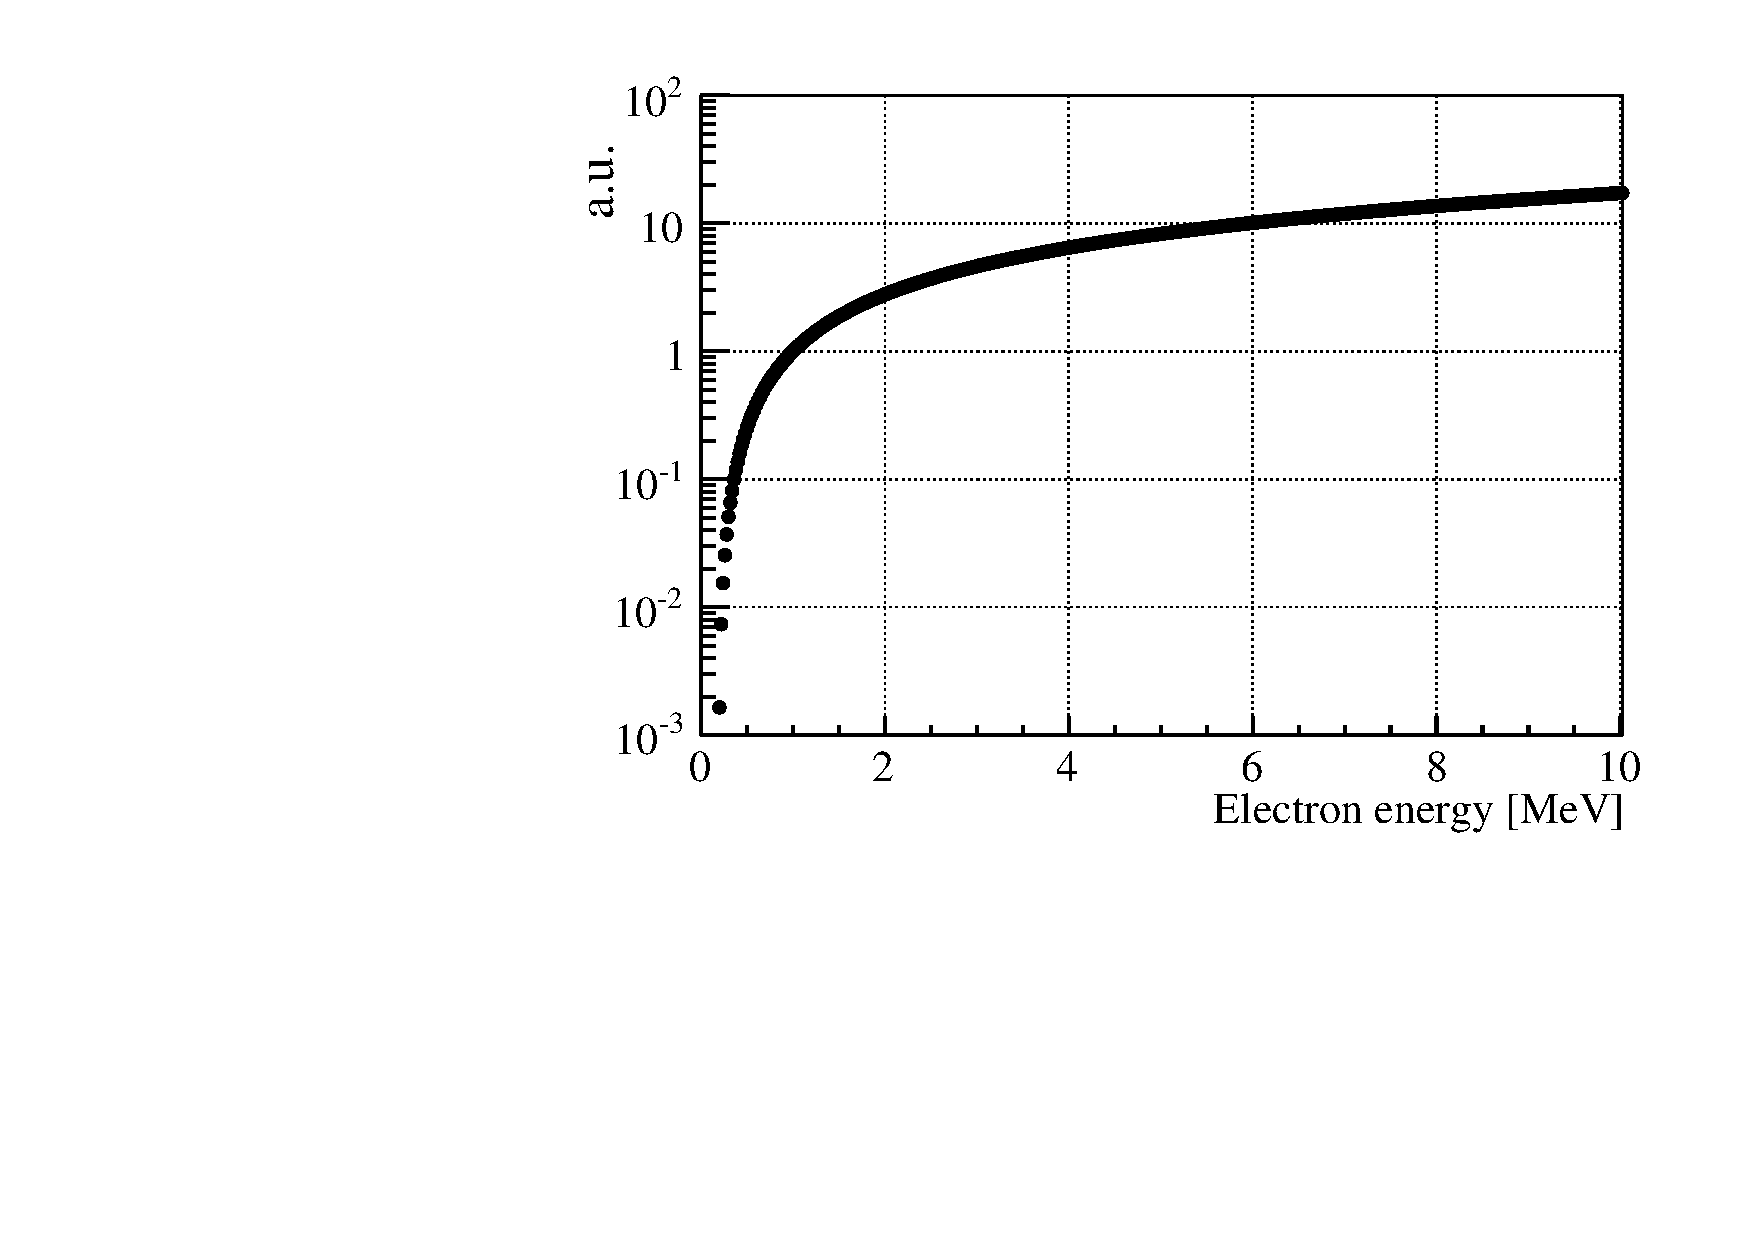
\includegraphics[scale=0.5]{Reconstruction/s04_CerenkonContribution.pdf}
  \caption{Energy dependence of the Cerenkov contribution to light emission by electrons in the LS (here, arbitrarily normalized at 1~MeV), from \cite{NonlinearityPaper}. The actual normalization of this function was determined by a fit to measurements of the nonlinearity, as described in \cite{NonlinearityPaper}.}
  \label{fig:cerenkovShape}
\end{figure}

Altogether, the combined effects on electrons of quenching and Cerenkov emission are therfore described by the relation
\begin{equation}
  \label{eq:reconScintNonlin}
  \frac{E_{\mathrm{vis},e^-}}{\Edepelec} = \beta_{\mathrm{vis}}[f_q(\Edepelec, k_B) + k_c f_c(\Edepelec)],
\end{equation}
where $f_q$ is given by \autoref{eq:reconBirksInt}, and $f_c$ (which, being tabulated from simulation data, cannot be expressed as an equation) is, again, shown in \autoref{fig:cerenkovShape}. Here, we have introduced the constant $k_c$, which describes the ratio of the amount of Cerenkov emission to scintillation. $\beta_{\mathrm{vis}}$ is an arbitrary normalization. The parameters $k_B$ and $k_c$ are determined from data, as will be described shortly.

Thus far we have only discussed the response of the scintillator to electrons. The end goal, however, is to characterize the response to positrons, since that is what will allow the measurement of the neutrino spectrum. Before the positron annihilates, it effectively ionizes the medium in the same manner as an electron would. Following ionization, we measure the response of the scintillator to two 511~keV gammas. Accordingly,
\begin{equation}
  \label{eq:reconScintPositron}
  E_{\mathrm{vis},e^+}(E_{\mathrm{kin}}) = E_{\mathrm{vis},e^-}(E_{\mathrm{kin}}) + 2 \times E_{\mathrm{vis},\gamma}(\SI{0.511}{MeV}).
\end{equation}

Gammas, in turn, do not themselves ionize, but they do produce and scatter electrons and positrons. The total response to gammas is, accordingly, rather complex, given the need to account for annihilation and pair production \emph{ad nauseam}. As such, Geant4 simulation were used to determine the response of the scintillator to gammas, as a function of $k_B$ and $k_c$. The (ionization) energy deposited by each simulated electron and positron was converted into visible energy according to \eqref{eq:reconScintNonlin}, and the sum gave the visible energy from each gamma. With the response to gammas thus determined, it could be plugged into \eqref{eq:reconScintPositron} to give the response to positrons.

In addition to the nonlinear light \emph{emission} of the scintillator, there is also nonlinear light \emph{measurement} caused by the design of the electronics. As was described in \autoref{sec:reconHitSelection}, the charge (i.e. light) in each channel is determined by taking the \emph{first} hit within the nominal time window. And as was described in \autoref{sec:calibHitCharge}, the first hit will tend to accurately measure the light observed by the PMT, \emph{provided that all of the photons arrived within 100~ns of each other.} However, some 5\% of the light is ``slow'' and will arrive too late to be captured by the hit that corresponds to the fast/medium light. Thus, high-energy events, in which every channel ``sees'' some fast/medium light, will fail to record any of the slow light. Conversely, in a lower-energy event, some of the slow light \emph{will} be recorded, since there is not enough fast/medium light to hit every channel. This means that the electronics response is slightly suppressed for high-energy events and slightly enhanced for low-energy ones.

Based on a combination of measurements and simulations, this behavior was found to be adequately described by the relation
\begin{equation*}
  \frac{\Erec}{\Evis} = \beta_{\mathrm{rec}}\left[ 1 + \alpha \left( - \frac{\Evis}{\tau} \right) \right],
\end{equation*}
where $\alpha$ and $\tau$ are, like $k_B$ and $k_c$, constrained by measurements, and $\beta_{\mathrm{rec}}$ is, like $\beta_{\mathrm{vis}}$, merely an arbitrary normalization. The product $\beta_{\mathrm{vis}}\beta_{\mathrm{rec}}$, by convention, is chosen to ensure that $\Erec = \Edep$ for 8~MeV electrons.

In order to determine the four parameters $k_B$, $k_c$, $\alpha$, and $\tau$ of the nonlinearity model, a fit was performed to a dataset consisting of the peaks from twelve gamma lines (both deployed and natural) as well as the electron spectrum from cosmogenic $^{12}$B decays, as shown in Figs XXX and XXX. The measured values of $\Erec$ were compared to those predicted by simulation (for a given set of the parameters), and the best-fit parameters were determined as those that minimized the $\chi^2$ between measurement and prediction. As no significant differences in nonlinearity were observed between ADs, a single nonlinearity model is used for all eight. The best-fit parameters were found to be $k_B = 15 \times 10^{-3}\;\mathrm{cm\, MeV^{-1}}$, $k_c = 0.5\%$, $\alpha = 0.078$, and $\tau = \SI{2.55}{MeV}$. However, these values depend on the assumed shapes $f_q$ and $f_q$, which in turn depend on the configuration of Geant4. Accordingly, our analysis does not make direct use of these four parameters; instead we directly use the digitized nonlinearity curve that they determine, as shown in Fig XXX, which includes a 1$\sigma$ uncertainty band on the scale of 1\%.

The scintillator nonlinearity was cross-checked using the 53~MeV Michel electron endpoint from muon decay as well as the $\beta+\gamma$ spectra from bismuth and thallium decays, while the electronics nonlinearity was validated using data from a fast ADC system that directly recorded the PMT waveforms in one AD. Further validation involved verifying that the best-fit model remained stable under removal of any single calibration point. The results of these studies were consistent with the 1\% 1$\sigma$ uncertainty band (derived from the $\chi^2$ fit) of the nonlinearity model.

\section{Vertex reconstruction}
\label{sec:reconVertex}

The AdSimple vertex reconstruction proceeds in multiple stages. First, an initial vertex is determined by taking a simple \emph{center of charge} (COC) using the coordinates of the PMTs. As this method suffers from significant biases (largely toward the center of the AD), a correction is then applied, based on interpolating a map of the mean bias (as a function of COC position) determined from a sample of Monte Carlo events, giving the \emph{Monte Carlo Corrected COC} (MCC-COC). However, even with the MC correction, this vertex still suffers from biases , particularly at large $z$, and there are additionally some observable ``wiggles'' in what should be uniform vertex distributions. In order to reduce such biases and clusterings, and also improve the resolution of the position reconstruction, a final vertex is computed by matching the distribution of PMT charges to a library of MC templates. We now discuss these steps in further detail. (XXX cite docs 7334 and 7536)


The COC vertex is calculated trivially,
\begin{equation*}
  x_{\mathrm{COC}} = \frac{\sum_{i}^{\mathrm{PMTs}} Q_i x_i}{\sum_i^{\mathrm{PMTs}} Q_i},
\end{equation*}
where $x_i$ is the position of the $i$th PMT, and $Q_i$ is the corresponding observed charge. To this vertex, the correction from MC is applied next.

The MC sample consists of a large number of uniformly-distributed IBD events, with (XXX presumably?) a spectrum that mimics the expected reactor spectrum. A cut is applied on the true interaction to eliminate events that occur outside the outer acrylic vessel. The positrons (i.e. prompt triggers) from these events are then used to generate correction table.

For each MC event, the COC vertex is calculated, and two corrections, a ``radial'' and a ``vertical'' one, are computed (using cylindrical coordinates):
\begin{equation*}
  \Delta r = \frac{\vec{r}_{\mathrm{true}} \cdot \vec{r}_{\mathrm{COC}}}{\abs{\vec{r}_{\mathrm{COC}}} - r_{\mathrm{COC}}},
\end{equation*}
\begin{equation*}
  \Delta z = z_{\mathrm{true}} - z_{\mathrm{COC}},
\end{equation*}
Events are divided into 20 bins for $0 < r_{\mathrm{COC}} < \SI{2}{m}$ and 40 bins for $-2 < z_{\mathrm{COC}} < \SI{2}{m}$. For each bin, the mean $\Delta z$ is computed, while the mean $\Delta r$ is computed over (and assigned to) all $z{_\mathrm{COC}}$ bins for a given $r_{\mathrm{COC}}$, since there is very little $z$ dependence on $\Delta r$. The $\Delta r$ and $\Delta z$ correction tables are ``pre-interpolated'' with a spline function to give a 10x-finer grid, which is then stored for use by AdSimple. During reconstruction, linear interpolation is applied to this fine-binned to look up the corrections for arbitary ($r_{\mathrm{COC}}$, $z_{\mathrm{COC}}$). Application of the correction is trivial: $r \mapsto r + \Delta r$ and $z \mapsto z + \Delta z$. This gives the MCC-COC vertex.

The final stage of the AdSimple vertex reconstruction relies on a library of 9,600 charge templates (i.e. distributions of charge across the PMTs), with each template corresponding to a cylindrical voxel of the detector. These voxels (i.e. bins) are defined as the product of 20 bins in $0 < r^2 < 2^2\;\mathrm{m}^2$, 20 bins in $-2 < z < \SI{2}{m}$, and 24 bins in $0 < \phi < 2\pi$. The charge template for each voxel is taken from the mean of the charge distributions (each normalized by total charge) of all MC events whose true position lay within the voxel. The MC sample, in turn, is of the same nature as the one used for the COC correction: reactor IBD positrons lying within the OAV. Taking advantage of the azimuthal symmetry of the detector response, each event was rotated in angular steps of $\pi/12$ to produce 23 ``clones'', which were added to the sample, thereby providing a ``free'' boost in statistics without the need to generate additional MC events.

\newcommand\Niobs{N_i^{\mathrm{obs}}}
\newcommand\Niexp{N_i^{\mathrm{exp}}}

During reconstruction, the charge templates are compared to the event's (normalized) charge distribution using the ``$\chi^2$'' (more precisely, the log-likelihood)
\begin{align*}
  \chi^2 &= \sum_i^{\mathrm{PMTs}}\left[ -2 \ln \frac{P(\Niobs, \Niexp(r^2, z, \phi))}
        {P(\Niobs, \Niobs)} \right] \\
      &= 2 \sum_i^{\mathrm{PMTs}} \left[ \Niexp - \Niobs+ \Niobs \ln \left( \frac{\Niobs}{\Niexp} \right) \right],
\end{align*}
where $P(n, \nu) = \nu^n e^{-n} / (n!)$, the Poisson probability of observing $n$ events when $\nu$ are expected. The MCC-COC vertex is used as a starting point to search the grid for a local minimum (which is presumably also a global minimum). Having thus located the bin with the lowest $\chi^2$, the reconstruction proceeds by quadratically interpolating the $\chi^2$ values at the neighboring grid points. This interpolation is performed independently for the three coordinates $r^2$, $z$, and $\phi$, each time using two neighbors in the appropriate direction. Letting $s$ denote any of the three coordinates, with $s_1$ being the value of $s$ at the $\chi^2$-minimizing grid point, and $s_2$ and $s_3$ being those of the neighbors, the value of $s$ at the interpolated minimum is
\begin{equation*}
  s_{\mathrm{min}} = \frac{(s_1^2 - s_2^2)(\chi_3^2 - \chi_1^2) - (s_1^2 - s_3^2)(\chi_2^2 - \chi_1^2)}{2(s_1 - s_2)(\chi_3^2 - \chi_1^2) - 2(s_1 - s_3)(\chi_2^2 - \chi_1^2)}.
\end{equation*}
Calculated in this manner, $r_{\mathrm{min}}$, $z_{\mathrm{min}}$, and $\phi_{\mathrm{min}}$ give the final AdSimple reconstructed vertex. This vertex provides a significantly improved resolution compared to the MCC-COC vertex, of $\sim$7~cm in $r$ and $\sim$9~cm in $z$, compared to 11.5 and 17~cm, respectively, for the MCC-COC. There are also no significant biases within the OAV region; although some high-frequency ``wiggles'' remain (as a consequence of the finite grid spacing), these are insignificant in the context of performing physics analysis, as shown, for instance, by the consistency of physics results between AdSimple and AdScaled (which lacks such structures).

Note that the reconstructed vertex is not directly used in selecting IBD candidates in this analysis. However, it is still used indirectly in calculating the reconstructed energy. In addition, some studies of background rates and spectra also depended on the reconstructed vertex. Finally, there is an indpendent oscillation analysis (not covered in this thesis), based on selecting IBDs where the neutron is captured on hydrogen, and this one typically relies on the use of the prompt-delayed distance in order to reduce the background of accidental coincidences.

\end{document}